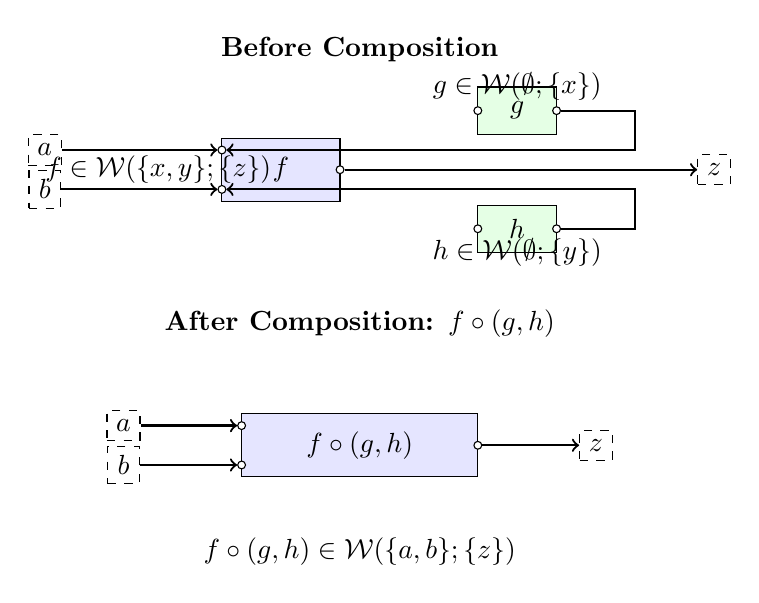
\begin{tikzpicture}[
  box/.style={rectangle, draw, minimum width=1.5cm, minimum height=0.8cm, fill=blue!10},
  subbox/.style={rectangle, draw, minimum width=1cm, minimum height=0.6cm, fill=green!10},
  wire/.style={->, thick},
  port/.style={circle, draw, fill=white, inner sep=1pt},
  interface/.style={rectangle, draw, dashed, minimum width=0.4cm, minimum height=0.25cm}
]

% Top diagram: Before composition
\node[above] at (0, 4) {\textbf{Before Composition}};

% Input interfaces
\node[interface] (in1) at (-4, 3) {$a$};
\node[interface] (in2) at (-4, 2.5) {$b$};

% Main operation f
\node[box] (f) at (-1, 2.75) {$f$};

% Sub-operations g and h
\node[subbox] (g) at (2, 3.5) {$g$};
\node[subbox] (h) at (2, 2) {$h$};

% Output
\node[interface] (out1) at (4.5, 2.75) {$z$};

% Ports for f
\node[port] (fp1) at (-1.75, 3) {};
\node[port] (fp2) at (-1.75, 2.5) {};
\node[port] (fq) at (-0.25, 2.75) {};

% Ports for g
\node[port] (gp) at (1.5, 3.5) {};
\node[port] (gq) at (2.5, 3.5) {};

% Ports for h  
\node[port] (hp) at (1.5, 2) {};
\node[port] (hq) at (2.5, 2) {};

% Wires
\draw[wire] (in1) -- (fp1);
\draw[wire] (in2) -- (fp2);
\draw[wire] (fq) -- (out1);
\draw[wire] (gq) -- (3.5, 3.5) -- (3.5, 3) -- (fp1);
\draw[wire] (hq) -- (3.5, 2) -- (3.5, 2.5) -- (fp2);

% Labels
\node[above] at (g) {$g \in \mathcal{W}(\emptyset; \{x\})$};
\node[below] at (h) {$h \in \mathcal{W}(\emptyset; \{y\})$};
\node[left] at (f) {$f \in \mathcal{W}(\{x,y\}; \{z\})$};

% Bottom diagram: After composition
\node[above] at (0, 0.5) {\textbf{After Composition: $f \circ (g, h)$}};

% Input interfaces for composed diagram
\node[interface] (cin1) at (-3, -0.5) {$a$};
\node[interface] (cin2) at (-3, -1) {$b$};

% Composed operation box
\node[box, minimum width=3cm] (comp) at (0, -0.75) {$f \circ (g, h)$};

% Output
\node[interface] (cout) at (3, -0.75) {$z$};

% Ports
\node[port] (cp1) at (-1.5, -0.5) {};
\node[port] (cp2) at (-1.5, -1) {};
\node[port] (cq) at (1.5, -0.75) {};

% Wires  
\draw[wire] (cin1) -- (cp1);
\draw[wire] (cin2) -- (cp2);
\draw[wire] (cq) -- (cout);

% Result notation
\node[below] at (0, -1.8) {$f \circ (g, h) \in \mathcal{W}(\{a,b\}; \{z\})$};

\end{tikzpicture}